
%==============================================================================
% Voorbeeld gebruik documentklasse hogent-article
%==============================================================================
%
% Compileren in TeXstudio:
%
% - Zorg dat Biber de bibliografie compileert (en niet Biblatex)
%   Options > Configure > Build > Default Bibliography Tool: "txs:///biber"
% - F5 om te compileren en het resultaat te bekijken.
% - Als de bibliografie niet zichtbaar is, probeer dan F5 - F8 - F5
%   Met F8 compileer je de bibliografie apart.
%
% Als je JabRef gebruikt voor het bijhouden van de bibliografie, zorg dan
% dat je in ``biblatex''-modus opslaat: File > Switch to BibLaTeX mode.

\documentclass{hogent-article}

%images
\usepackage{graphicx}
\graphicspath{ {./img/} }

%------------------------------------------------------------------------------
% Metadata over het artikel
%------------------------------------------------------------------------------

%---------- Titel & auteur ----------------------------------------------------
\PaperTitle{Heeft de factor muziek invloed op de resultaten van de retrieval practice studiemethode?}
% Dit is typisch de opdracht en het vak waarvoor dit artikel geschreven is, bv.
% ``Verslag onderzoeksproject Onderzoekstechnieken 2018-2019''
\PaperType{Verslag onderzoeksproject Onderzoekstechnieken 2018-2019}

\Authors{Olivier Troch\textsuperscript{1}, Daan Van Vooren \textsuperscript{2}, Robbie Verdurme\textsuperscript{3}, Sebastien Wojtyla\textsuperscript{4}} % Authors



% Als het hier gaat om een voorstel voor de bachelorproef, dan ben je hier
% verplicht de naam van je co-promotor in te vullen. Zoniet, dan kan je het
% leeg laten.
\CoPromotor{}

% Contactinfo: Geef hier de contactgegevens van elke auteur van het artikel (en
% indien van toepassing ook van de co-promotor).
\affiliation{
	\textsuperscript{1} \href{mailto:Olivier.troch.w2257@student.hogent.be}{Olivier.troch.w2257@student.hogent.be}
}
\affiliation{
	\textsuperscript{2} \href{mailto:daan.vanvooren.y1502@student.hogent.be}{daan.vanvooren.y1502@student.hogent.be}
}
\affiliation{
	\textsuperscript{3}
	\href{mailto:robbie.verdurme.y9234@student.hogent.be}{robbie.verdurme.y9234@student.hogent.be}
}
\affiliation{
	\textsuperscript{4}
	\href{mailto;sebastien.wojtyla.y3274@student.hogent.be}{sebastien.wojtyla.y3274@student.hogent.be}
}
%---------- Abstract ----------------------------------------------------------
\Abstract{In deze paper wordt onderzocht wat de effecten zijn op de resultaten van de retrieval practice studiemethode.
	In veel studies werd reeds aangetoond dat retrieval practice een goede studiemethode is maar welke factoren hierop invloed hebben is minder besproken. De paper gaat dieper in op deze vraag door te onderzoeken of het beluisteren van muziek gedurende de retrieval practice methode enige invloed zal hebben op de resultaten.
	De te verwachte resultaten zijn dat het beluisteren van muziek tijdens de retrieval practice studiemethode een negatief effect zullen hebben. Deze paper kan bijdragen aan verder onderzoek van de retrieval practice methode.
}

%---------- Onderzoeksdomein en sleutelwoorden --------------------------------
\Keywords{Onderzoeksproces, Studiemethodes, Retrieval Practice}
\newcommand{\keywordname}{Sleutelwoorden} % Defines the keywords heading name

%---------- Titel, inhoud -----------------------------------------------------

\begin{document}
	
	\flushbottom % Makes all text pages the same height
	\maketitle % Print the title and abstract box
	\tableofcontents % Print the contents section
	\thispagestyle{empty} % Removes page numbering from the first page
	
	%------------------------------------------------------------------------------
	% Hoofdtekst
	%------------------------------------------------------------------------------
	
	\section{Inleiding}
	Retrieval practice is een studiemethode die ervoor zorgt dat leerstof langer onthouden kan worden op lange termijn. Hoewel reeds aangetoond werd dat dit een effectieve methode is voor het studeren verwachten wij een ander resultaat wanneer we een variabele aanpassen. De variabele die wij hebben onderzocht in deze paper is het effect van muziek in combinatie met retrieval practice tijdens het instuderen van een tekst.
	
	\section{Overzicht literatuur}
	
	% Refereren naar de literatuur kan met:
	% \autocite{BIBTEXKEY} -> (Auteur, jaartal)
	% \textcite{BIBTEXKEY} -> Auteur (jaartal)
	% Voorbeeld van een referentie~\autocite{Moore2002}
	
	
	
	\section{Methodologie}
	De variabele die getest werd in deze paper is het effect van muziek beluisteren tijdens de retrieval practice methode.
	Door het beluisteren van muziek tijdens het instuderen kan het brein meer gestimuleerd worden. Hierdoor zal het brein ook de studiematerie kunnen linken aan de geluisterdde liederen en zo gemakkelijker de nieuwe materie onthouden.
	Dit kan een grote invloed hebben op het studeren zoals reeds bewezen is \autocite{ChanEtAl1998}.
	


	
	\section{Experimenten}
	Tijdens het onderzoek kreeg iedere informatica student een tekst over darwin die hij/zij zal moest bestuderen. Vervolgens werden de studenten opgesplitst in vier subgroepen. Elke subgroep werd gedifferentieerd op basis van het wel of niet luisteren naar muziek en het wel of niet toepassen van de retrieval practice methode.
	De eerste subgroep heeft de standaard retrieval practice methode toegepast zonder aangepaste variabele. 

	De tweede subgroep heeft naar muziek geluisterd tijdens het instuderen van de tekst. In combinatie met deze variable muziek werd er nog steeds gewerkt met de retrieval practice methode.
	
	De derde subgroep heeft ook naar muziek geluisterd tijdens het instuderen van de tekst maar zonder het toepassen van de retrieval practice methode.
	
	De vierde kreeg geen muziek te horen krijgen tijdens het instuderen van de tekst en ging dan ook niet te werk aan de hand van de retrieval practice methode.
	
	Hierdoor kon nagegaan worden of de variabele een invloed heeft op het studeren van een tekst aan de hand van de retrieval practice methode. Merk op dat we elke tweedejaars informatica student er toe verplichtten om deel te nemen aan deze test waardoor het resultaat niet op de hele groep studenten toepasbaar is zonder enig foutpercentage \autocite{karpicke2009metacognitive}.
	
	\section{verwachtingen}
	We veronderstellden dat de eerste subgroep analoge resultaten ging behalen aan de resultaten uit de artikels over de retrieval practice methode \autocite{butler2010repeated, pyc2012test, karpicke2007repeated, karpicke2008critical}. Dit omdat deze methode reeds vaak getest werd in verschillende experimenten.
	
	Daarnaast verwachtten we dat het beluisteren van muziek een negatief effect ging hebben op het resultaat. Door het beluisteren van muziek kan je sneller afgeleid graken tijdens het lezen van de tekst en deze dan ook minder gemakkelijk onthouden.
	
	\section{Analyse resultaten}
	\subsection{Retrieval Practice}
	In vergelijking met het artikels over de retrieval practice \autocite{butler2010repeated, pyc2012test, karpicke2007repeated, karpicke2008critical} liggen onze uitslagen toch wel dicht bij die van de artikels. Dit houd in dat we kunnen bewijzen dat de retrieval practice een aangeraden studie methode is met een hoge studie efficiëntie.
	
	%met rt en zonder rt vergelijken
	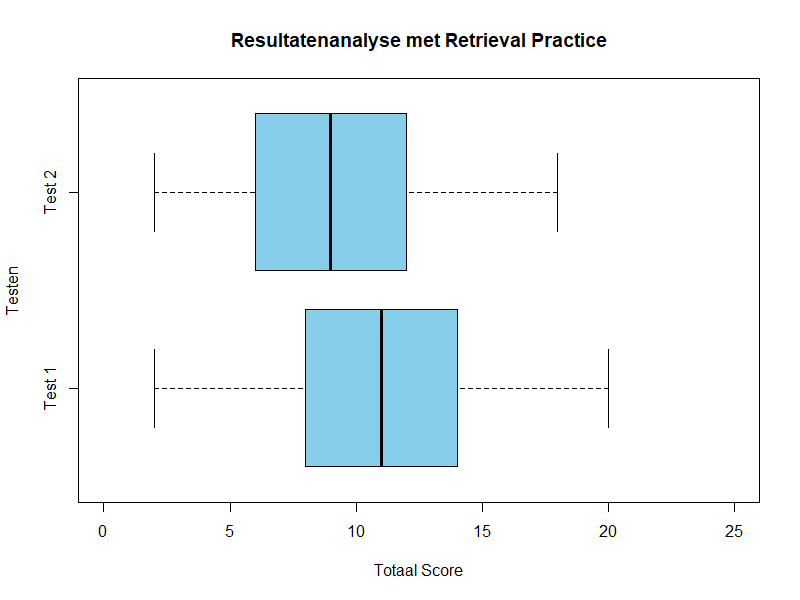
\includegraphics[width=120px]{Rplot_MetRetrievalPractice}
	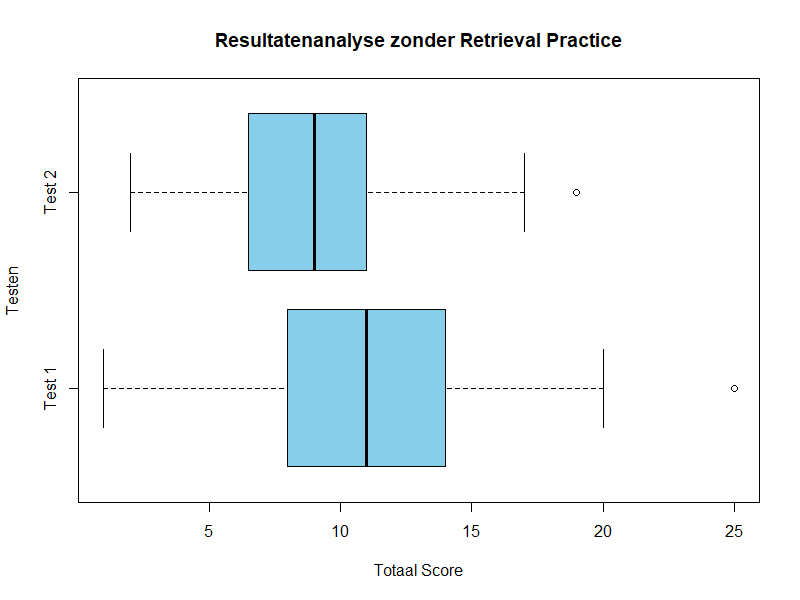
\includegraphics[width=120px]{Rplot_ZonderRetrievalPractice}
	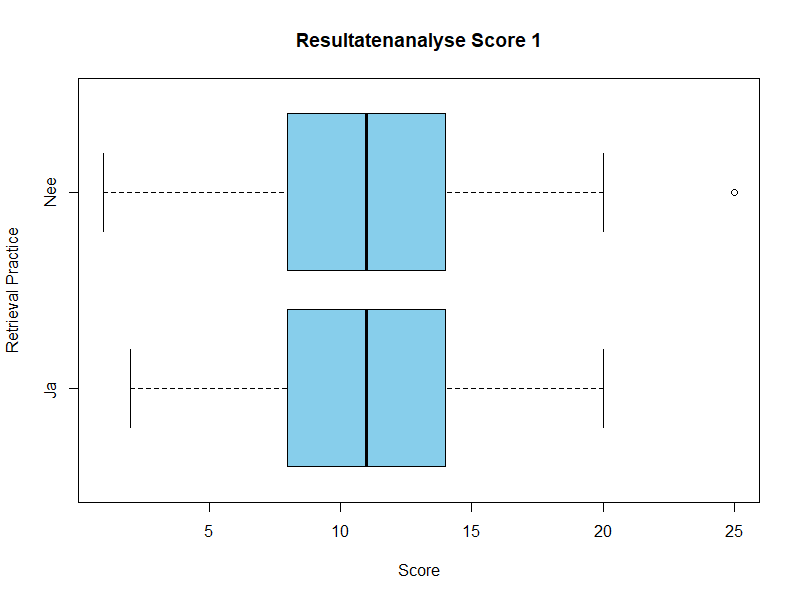
\includegraphics[width=120px]{Rplot_RetrievalPractice_Score1}
	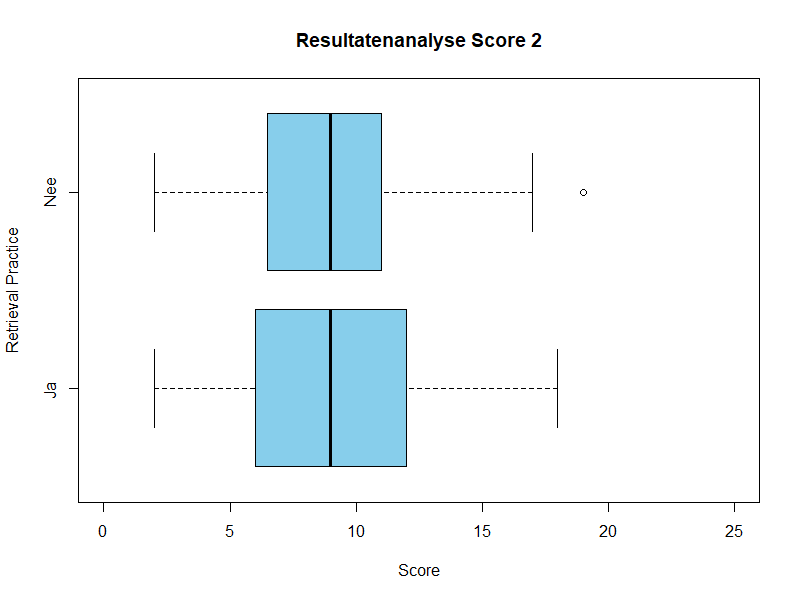
\includegraphics[width=120px]{Rplot_RetrievalPractice_Score2}
	Vanuit de testen blijkt dat de groep die de retrieval practice methode toepaste en de groep die dit niet deed de score niet significant verschillend is. De groep die de retrieval practice toepaste had net iets meer onthouden van de ingestudeerde tekst. Hieruit kunnen we de bevestigen wat de opgezochte artiekels beweren over het toepassen van de retrieval practice.
	
	\subsection{Muziek}
	%met muziek en zonder muziek vergelijken
	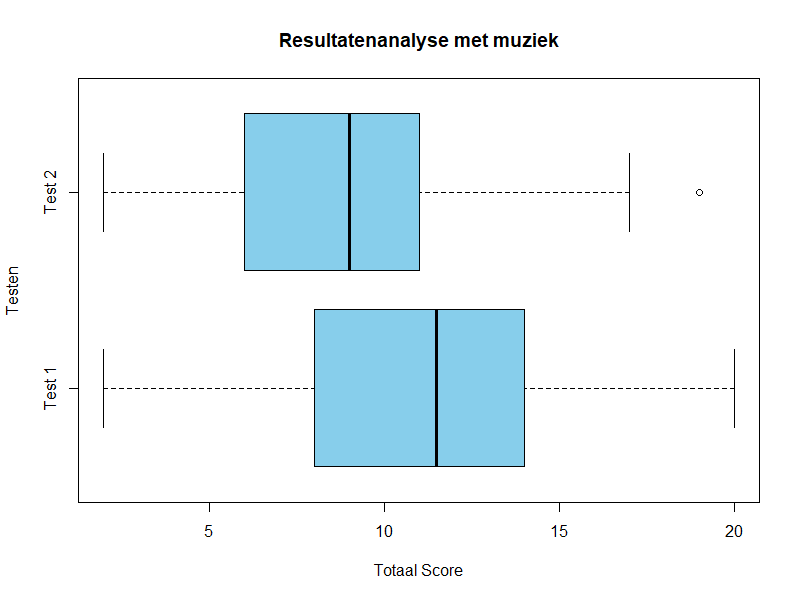
\includegraphics[width=120px]{Rplot_MetMuziek}	
	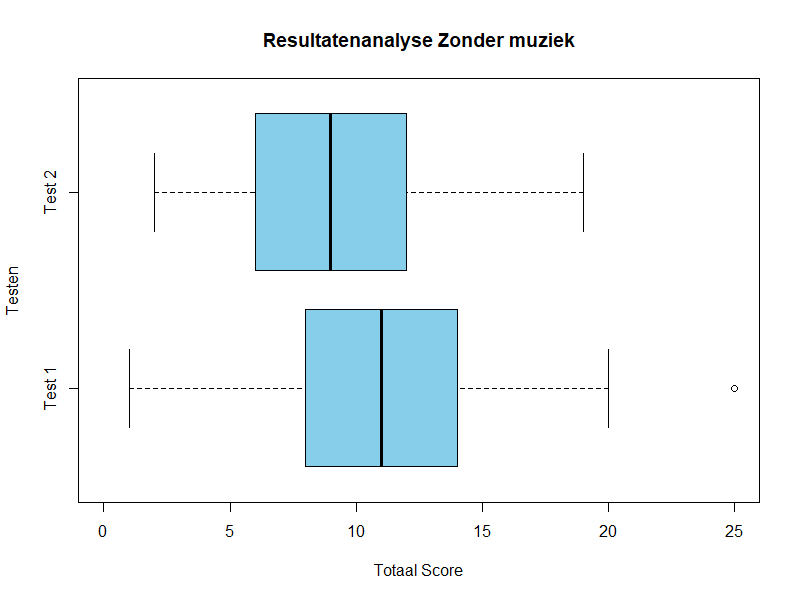
\includegraphics[width=120px]{Rplot_ZonderMuziek}
	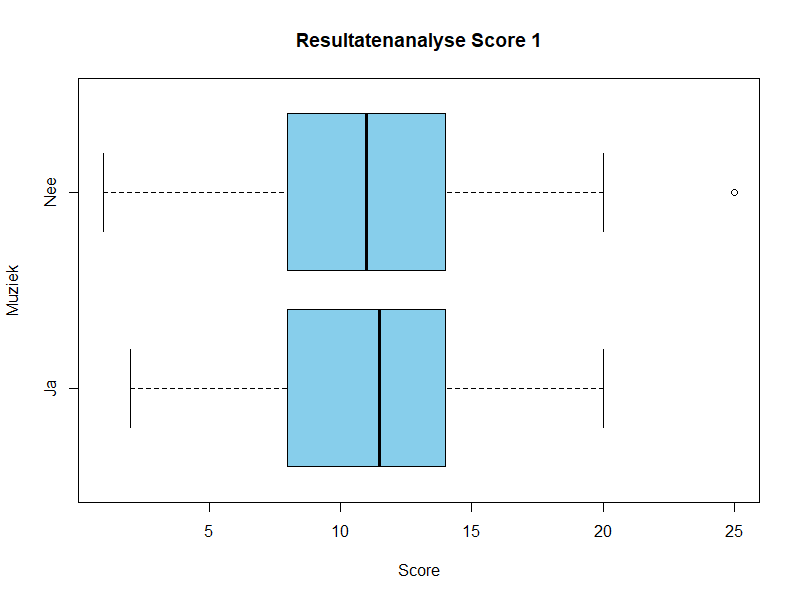
\includegraphics[width=120px]{Rplot_Muziek_Score1}
	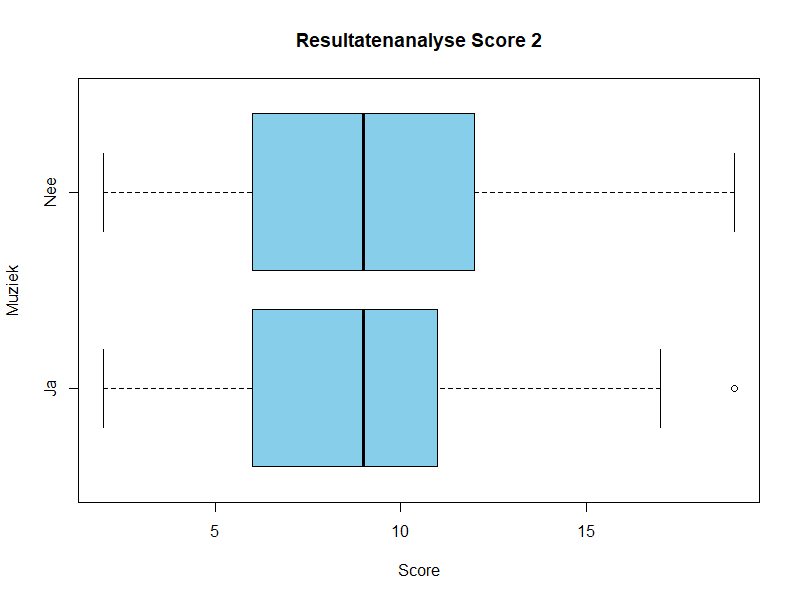
\includegraphics[width=120px]{Rplot_Muziek_Score2}
	Verder hebben we gekeken in deze paper naar de impact van het beluisteren van muziek tijdens het instuderen. Uit de testen dat we afgenomen hebben is er wel degelijk een significant verschill tussen het beluisteren van muziek. De groep die geen muziek beluisterde tijdens het instuderen behaalde een hogere score. Dit is zoals we enigsins verwacht hadden in deze paper. Dit kan het resultaat zijn van de muziek die teveel afleid tijdens het lezen en instuderen van de tekst.
	
	\subsection{Retieval Practice met Muziek}
	%met rt en muziek vergelijken
	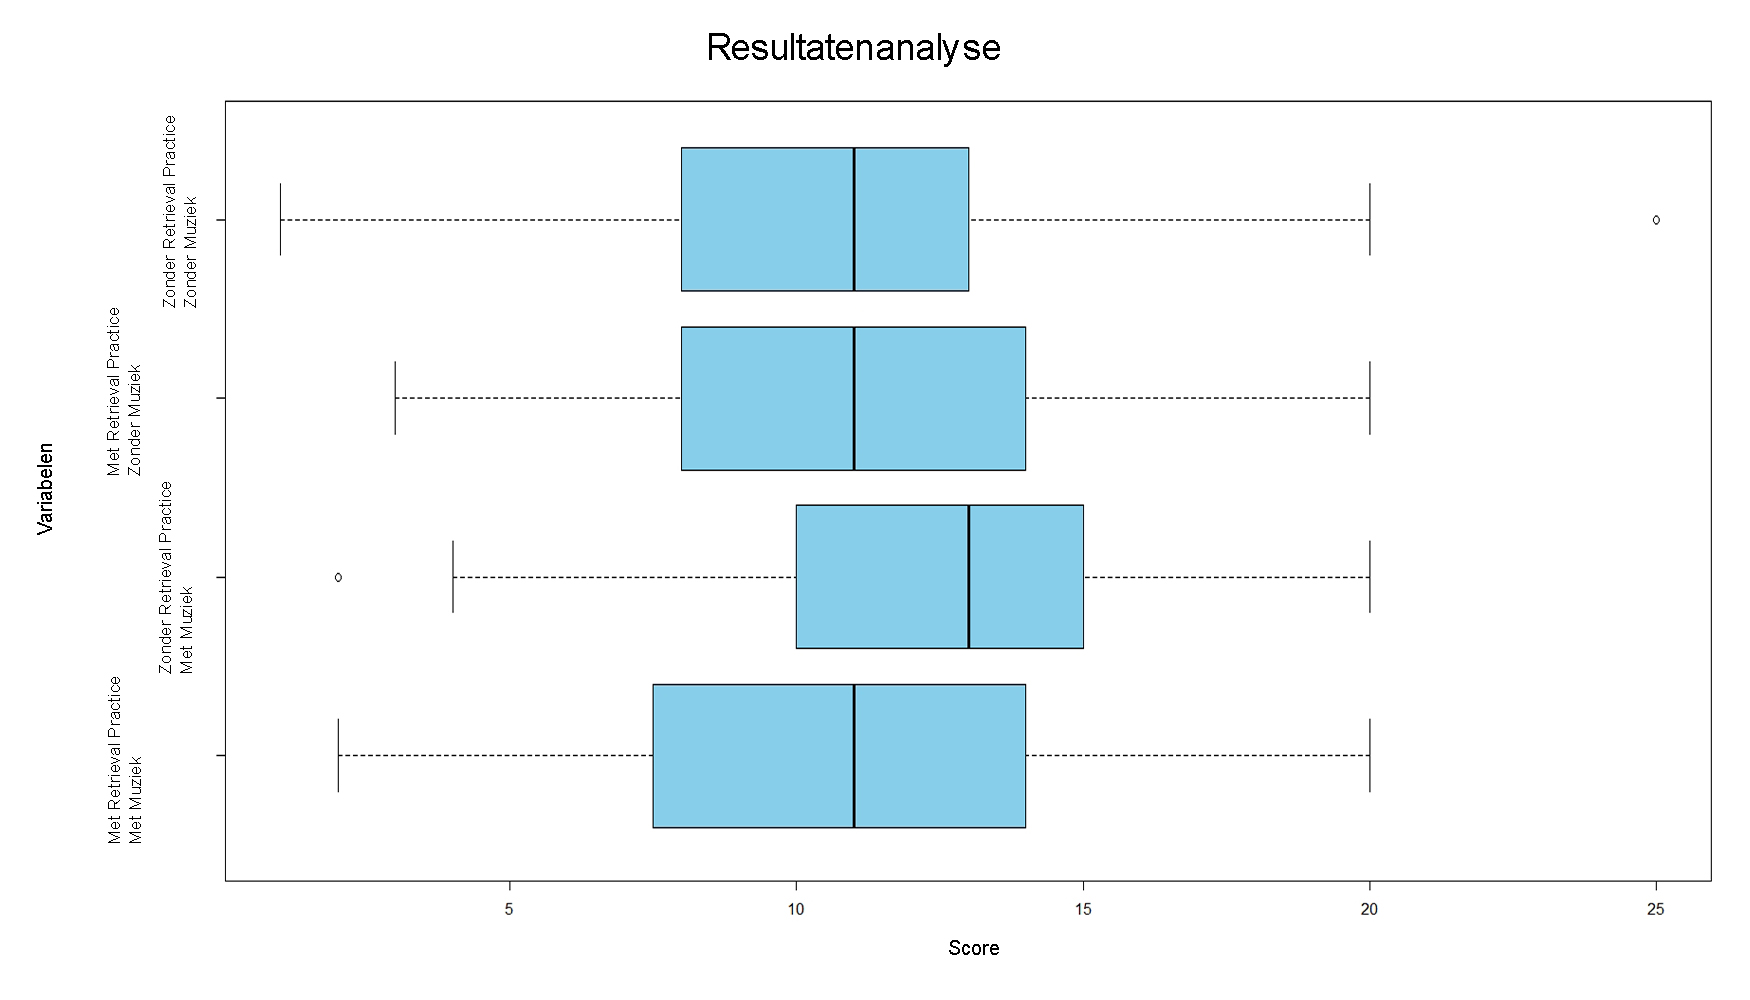
\includegraphics[width=120px]{Rplot_RetrievalPracticeMuziek_Score1}	
	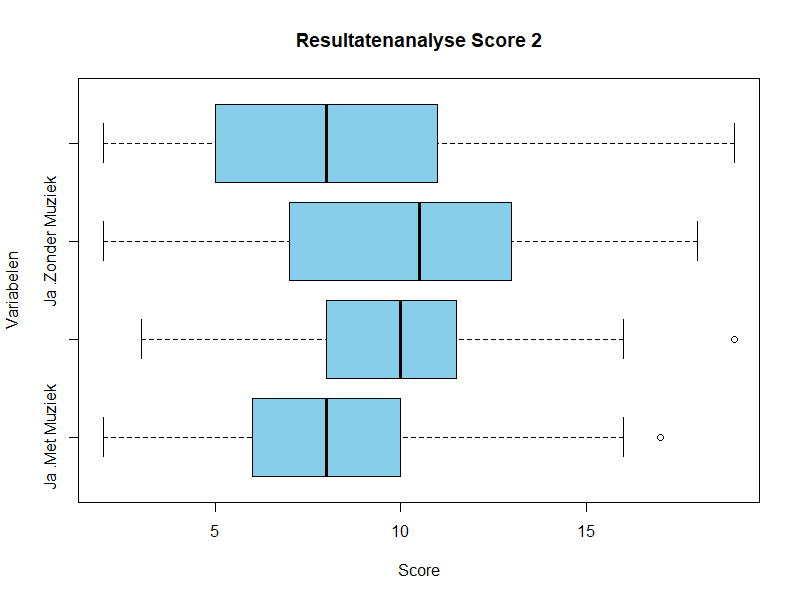
\includegraphics[width=120px]{Rplot_RetrievalPracticeMuziek_Score2}
	Als laaste vergelijking hebben we alle variablen vergeleken. Hieruit bleek dat de groep die zonder de retrieval practice en zonder de muziek de tekst ingestudeerd heeft beter te scoren in de test. Hieruit kun je afleiden dat de personen die op hun eigen manier de tekst instuderden zonder de afleiding van de muziek het beste de tekst konden reconstruweren.
	Uit deze boxplotten kunnen we ook afleiden dat het beluisteren van muziek een heel grote impakt heeft op het instuderen van de tekst. Deze variable heeft zelfs meer impakt dan het toepassen van de retrieval practice methode.  
	
	\section{Conclusie}
	Uit de resultaten van deze paper kunnen we concluderen dat het effect van muziek een grotere impakt heeft dan het toepassen van de retrieval practice. Dit is omdat de muziek je afleid als je dit niet op de juiste manier toepast en implementeerd is in je studiegedrag zoals in het artikel \autocite{ChanEtAl1998}. Dit kan enerzijds ook zijn doordat we de informatica studenten verplicht hebben om de retrieval practice methode toe te passen in plaats van hun eigen studie methodes die de testpersoon al reeds kent en gebruikt in het dagelijkse leven. Anderzijds kan het ook zijn door doordat de verbeterings criteria niet meegegeven zijn aan de studenten. Hierdoor konden ze niet goed inschatten op wat ze zouden verbeterd worden. Hierdoor kunnen we geen definitieve conclusies afleiden van de resultaten van deze opdracht.
	
	%------------------------------------------------------------------------------
	% Referentielijst
	%------------------------------------------------------------------------------
	% voorkomen. Gebruik JabRef om je bibliografie bij te houden en vergeet niet
	% om compatibiliteit met Biber/BibLaTeX aan te zetten (File > Switch to
	% BibLaTeX mode)
	
	\phantomsection
	\printbibliography[heading=bibintoc]
	
\end{document}
